So far we have shown how sustained CW-NIR laser affects neural activity by modifying the dynamics of spike generation. In the previous section \ref{sec:laser models} we used a conductance-based model to theoretically assess the spike evolution and the different candidates involved in the modulation of the action potential generation (i.e., ionic channels and capacitance). To address this effect in an experimental setting is a complex task. Usually, it is accomplished using chemicals to block or open specific channels \parencite{liang_temperature-dependent_2009}. This is not a generalizable method in different systems and individuals, and it restricts the channel study to a system with a detailed description of the specific neuron being recorded. We chose instead to assess the spike generation dynamics at different stages, which implies modifying the activity of several channels at a time in a precise timing relative to the spike generation dynamics. This task is only experimentally feasible with an activity-dependent stimulation protocol.

In infrared stimulation literature, the most spread technique has been pulsed illumination which stimulates at a fixed frequency. Although this approach has been effective in some tasks such as eliciting neural activity, it has limited possibilities in the context of precision and adaptability. Thus, with the activity-dependent protocol proposed here, we also provide an open-access alternative to the widely-used fixed-frequency pulsed laser stimulation protocols, which usually depend on a specific combination of restrictions from manufacturers, controllers, and diode laser availability. In addition, a closed-loop approach provides further means to deal with the history-dependent nature of neural dynamics and its partial observability \parencite{varona_online_2016}. 

In this section we present a new protocol for closed-loop stimulation, we first validate the hypothesis in the CGC-model, by modifying some channels conductance only during depolarization or repolarization phase, and then test the protocol in a experimental environment, controlling the laser illumination by a mechanical shutter. 


\subsection{Model simulation of activity-dependent stimulation}

To address in a computational approach the observed effect experimentally, we have simulated the effect on a CGC-model neuron modulating two of the channels where the effect on the neurons was larger. This way, only during a certain time interval, the conductance in channels gD and gHVA was modified to the value replicating hte "maximum effect" (see Figure \ref{fig:activity dependent model stimulation})

\begin{figure}[htb!]
	\centering
	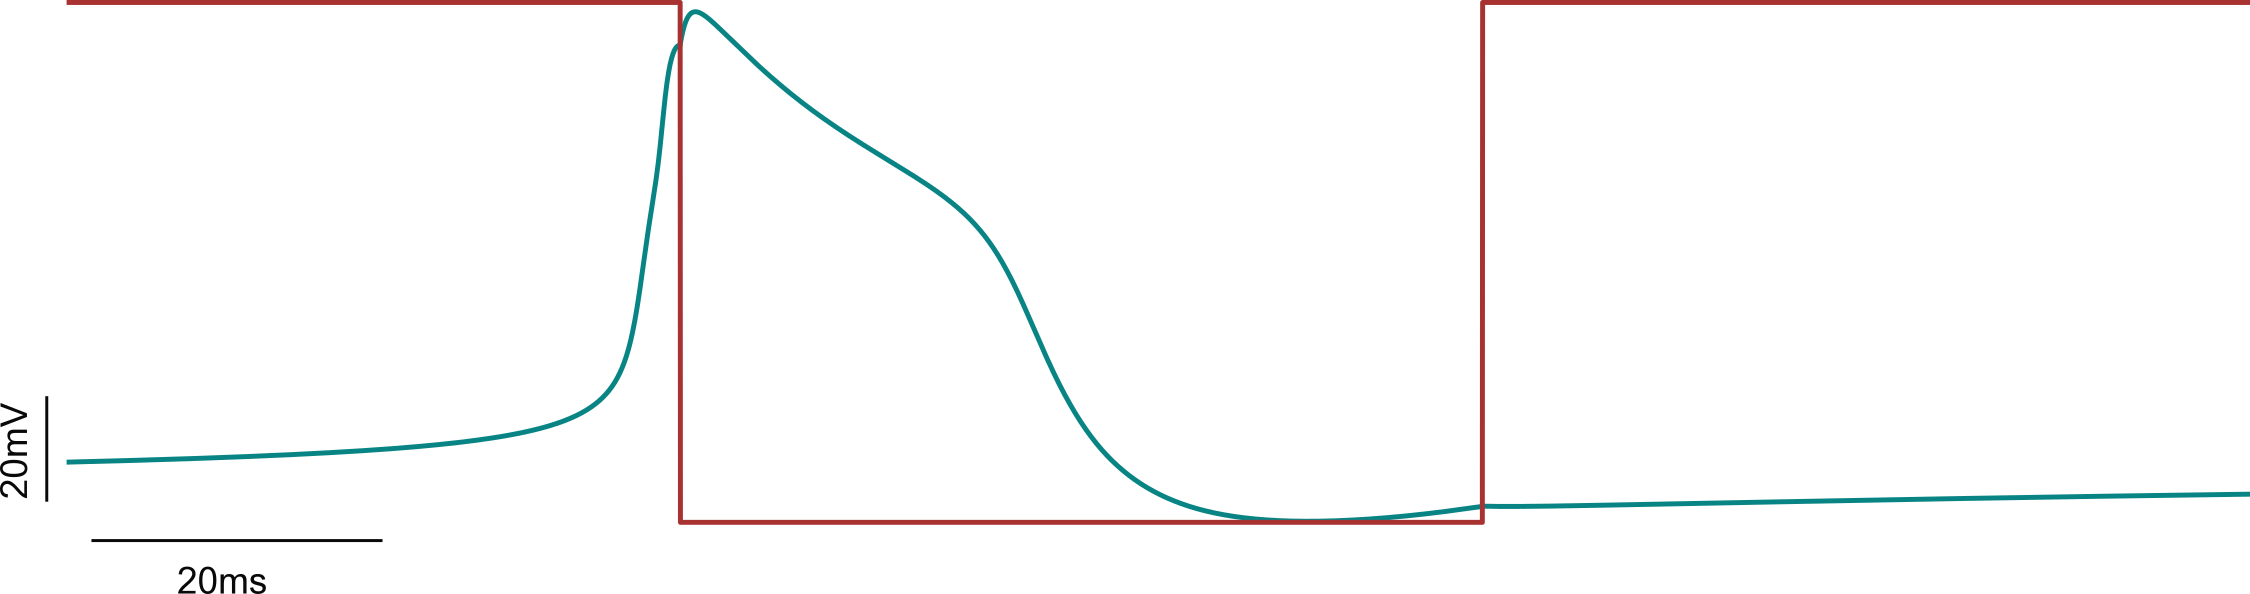
\includegraphics[width=0.7\textwidth]{img/laser/activity-dependent-model/depol_model.png}
	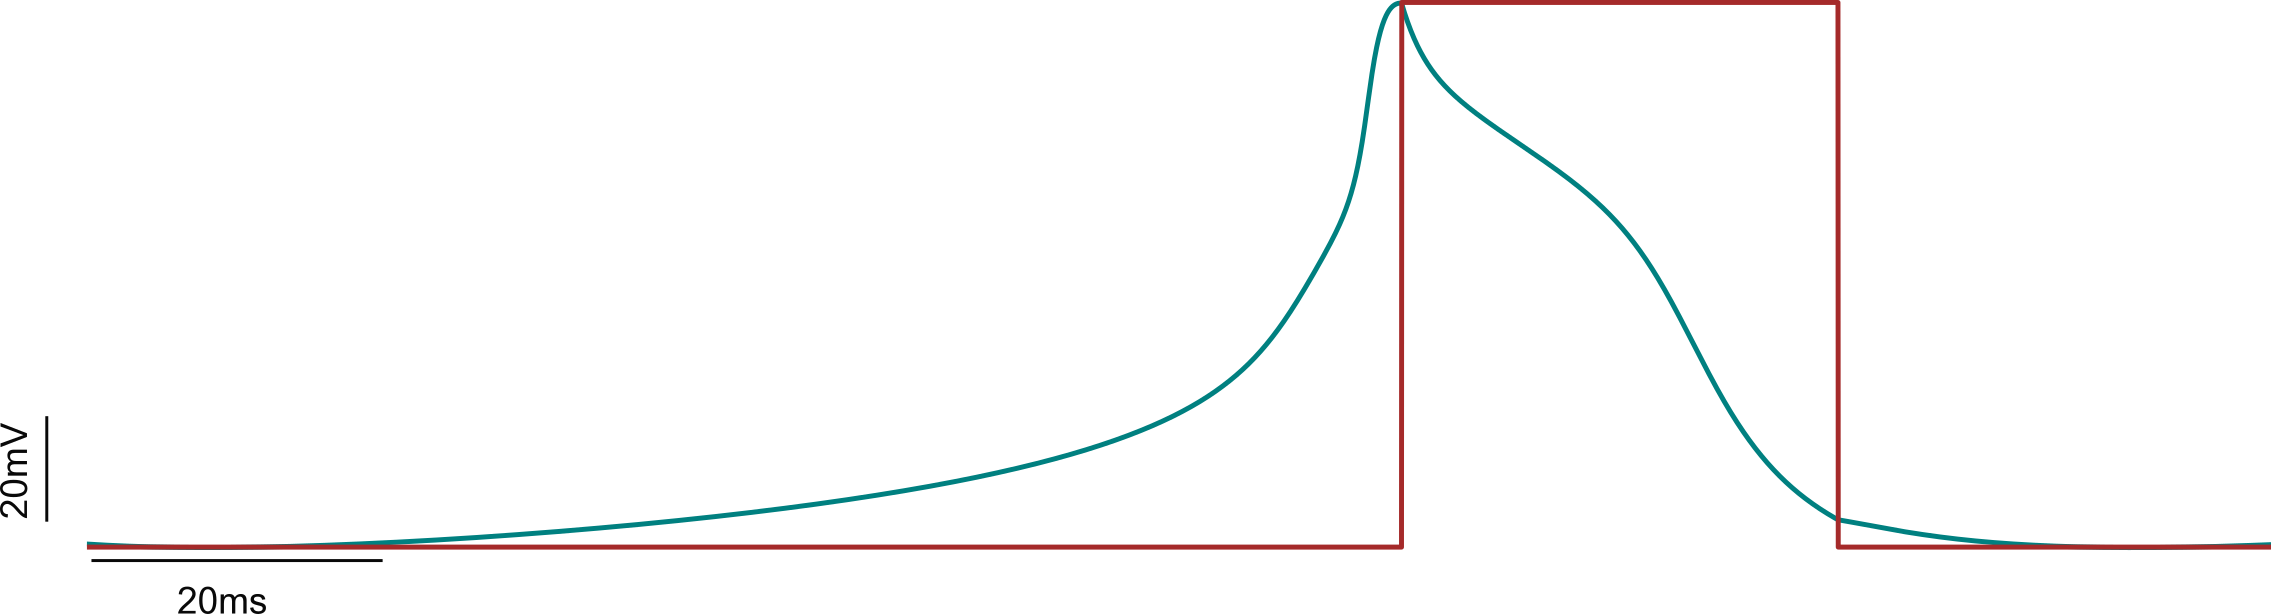
\includegraphics[width=0.7\textwidth]{img/laser/activity-dependent-model/repol_model.png}
	\caption{Simulation of the effect of CW-NIR laser in the CGC-model. Stimulating only during the depolarization or only during repolarization phases for first and second rows respectively.}
	\label{fig:activity dependent model stimulation}
\end{figure}

With this simulation we obtained the results showed in Figure \ref{fig:activity dependent simulation results}, where, as in the experimental results, the effect is larger when the stimulation is only in the repolarization slope, whereas while the effect is over the depolarization slope, the effect is only visible in the depolarization slope. 

\begin{figure}[htb!]
	\centering
	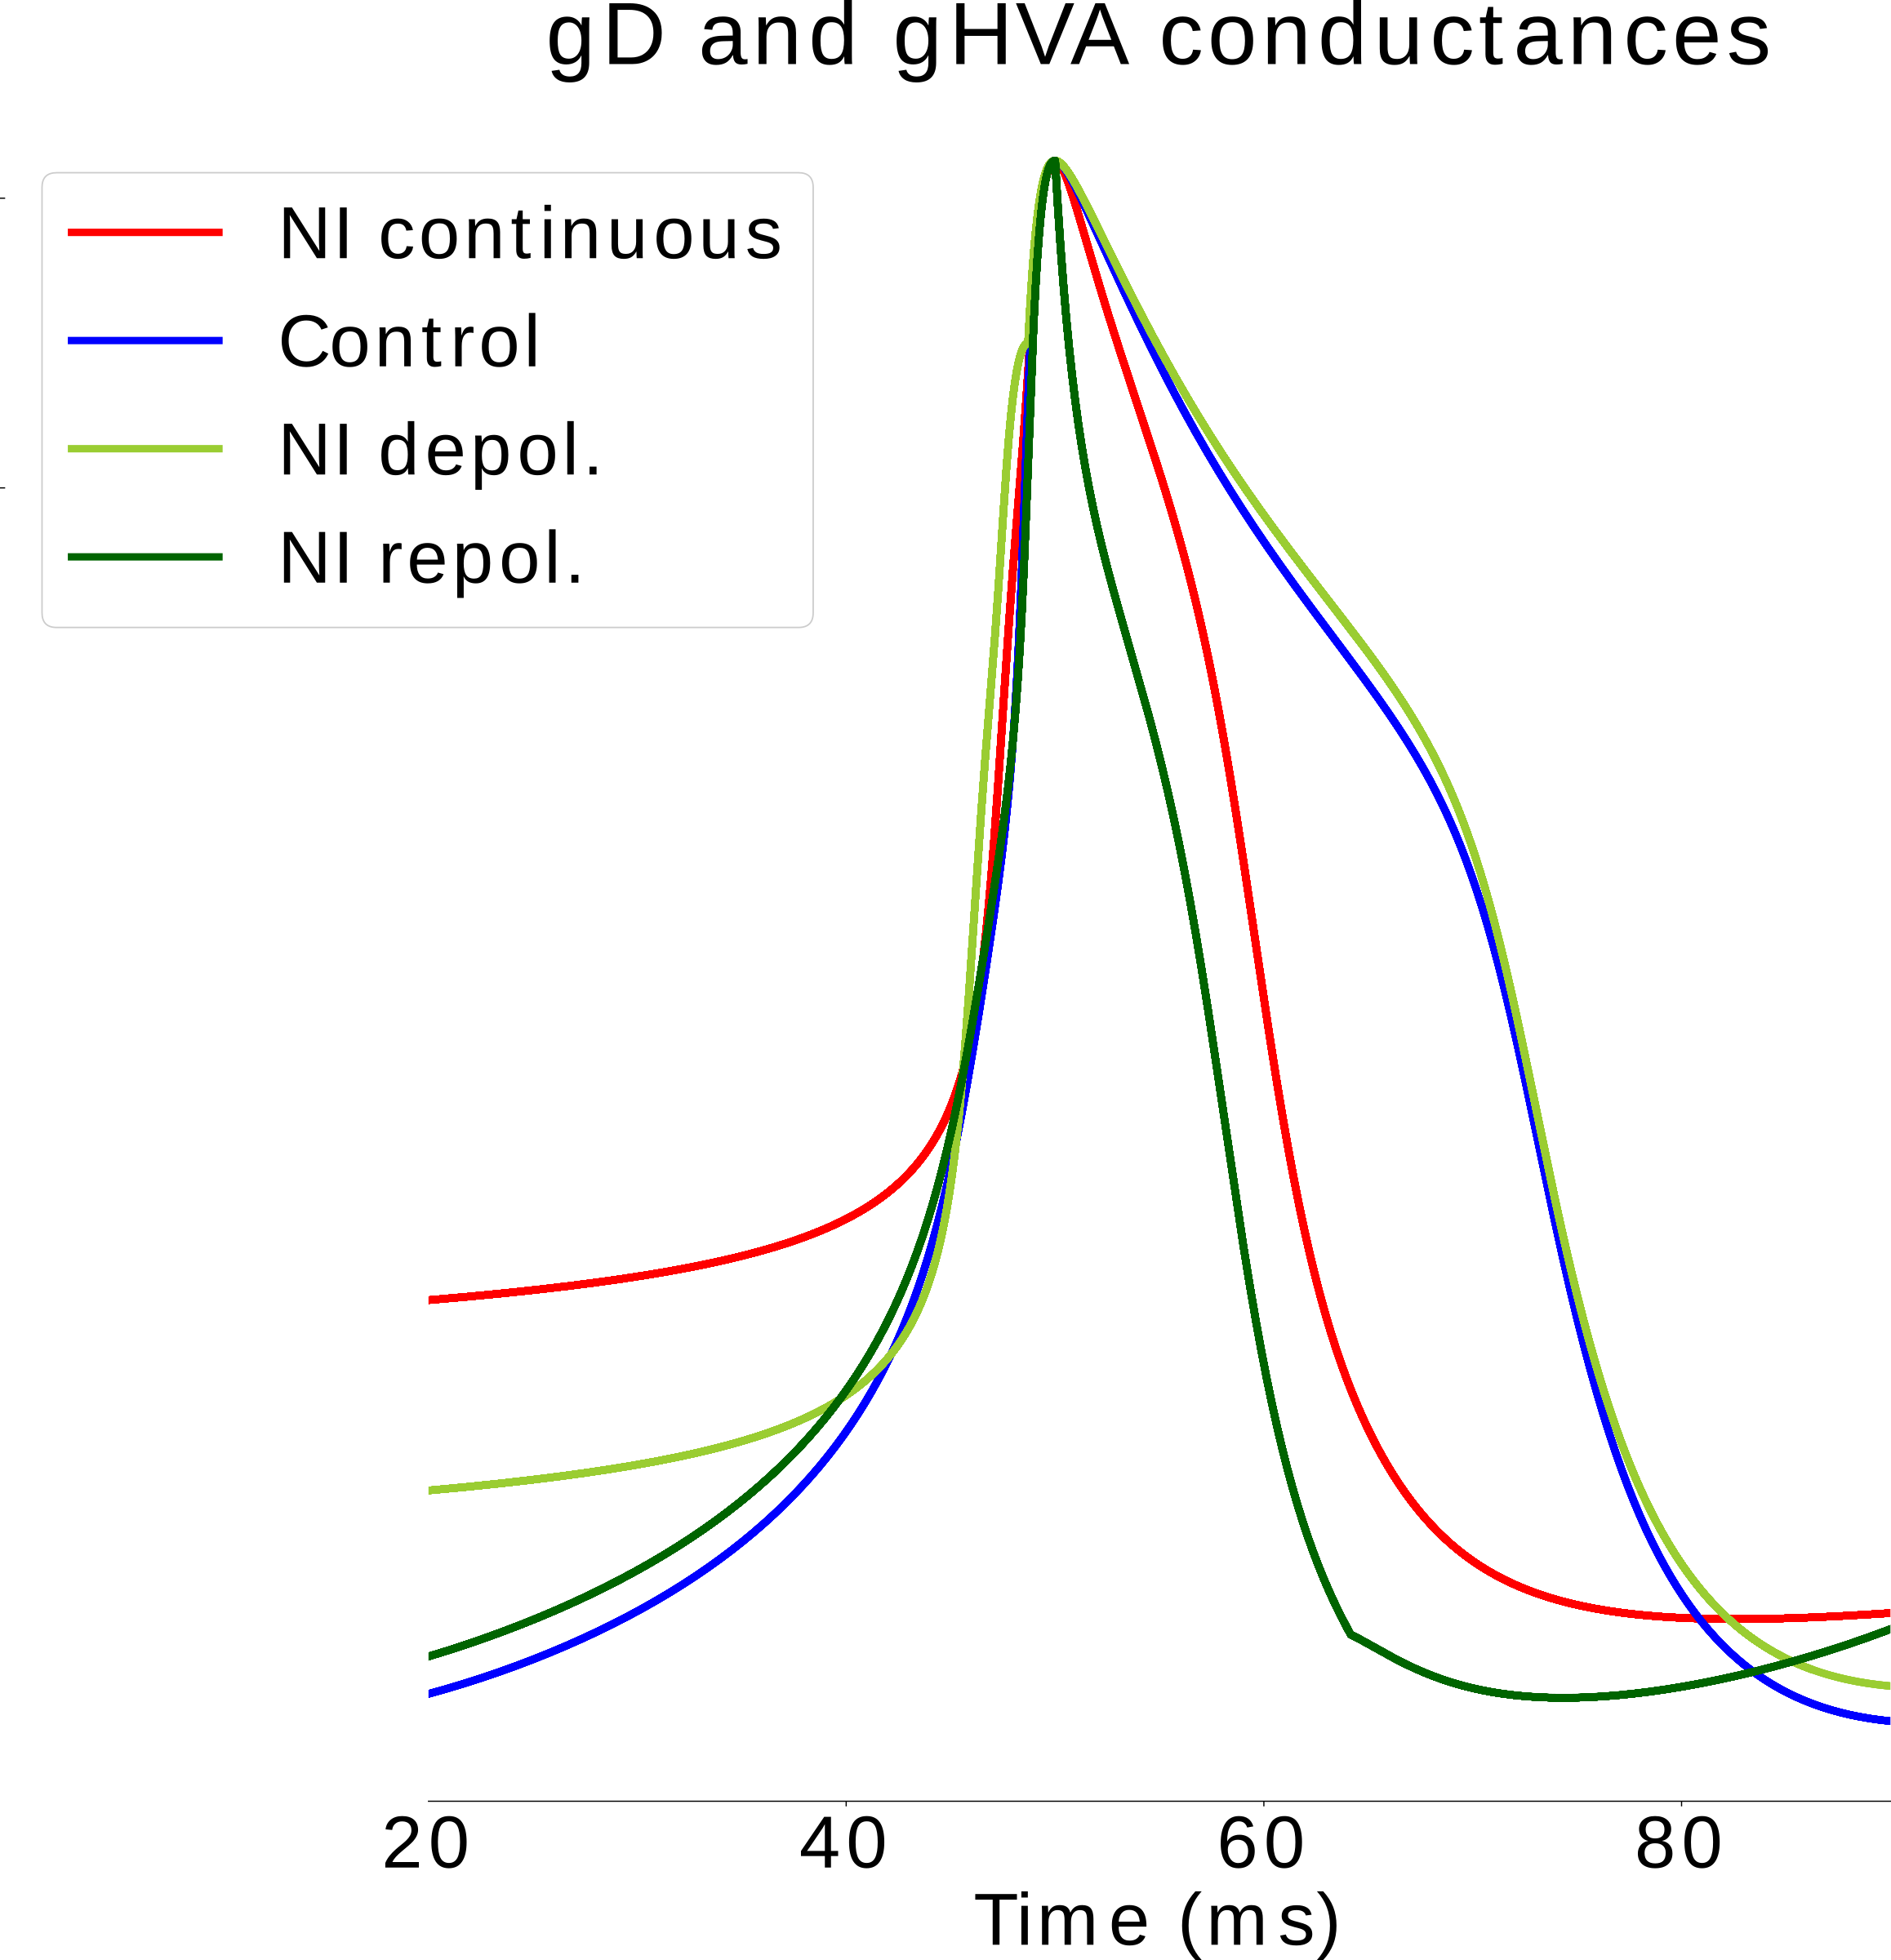
\includegraphics[width=0.5\textwidth]{img/laser/activity-dependent-model/depol_combined.png}
	\caption{Results in the spike waveform for the simulation of the effect of CW-NIR laser in the CGC-model. Stimulating only during the depolarization or only during repolarization phases for first and second rows respectively.}
	\label{fig:activity dependent simulation results}
\end{figure}

\subsection{Experimental activity-dependent stimulation}

Here we propose a closed-loop stimulation protocol where we can differentiate between the phases of the action potential and illuminate the neurons only at certain intervals of the spike generation dynamics. In this protocol, the laser illumination was controlled by a mechanical shutter triggered by the prediction of events in the voltage signal. A real-time software system ran the prediction algorithm and triggered the illumination for short periods of time at different phases of the spike generation when distinct channels were active (see Sec. \ref{sect:methods-activity-dependent} and Fig. \ref{fig:activity dependent protocol}). The prediction of the events was computed by two algorithms, one based on a voltage threshold updated at each spike peak occurrence and a second one that calculated the voltage area from the hyperpolarization (minimum) to the next hyperpolarization. Based on this prediction the illumination was triggered at the specified time before the spike occurrence (see Sec. \ref{sect:methods-activity-dependent} for details in these algorithms). The implementation of these algorithms is available as a module for the real-time open-source system RTXI \parencite{patel_hard_2017} in \href{github.com/GNB-UAM/spike_predictor}{https://github.com/GNB-UAM/spike\_predictor}.

\begin{figure}[htb!]
	\centering
	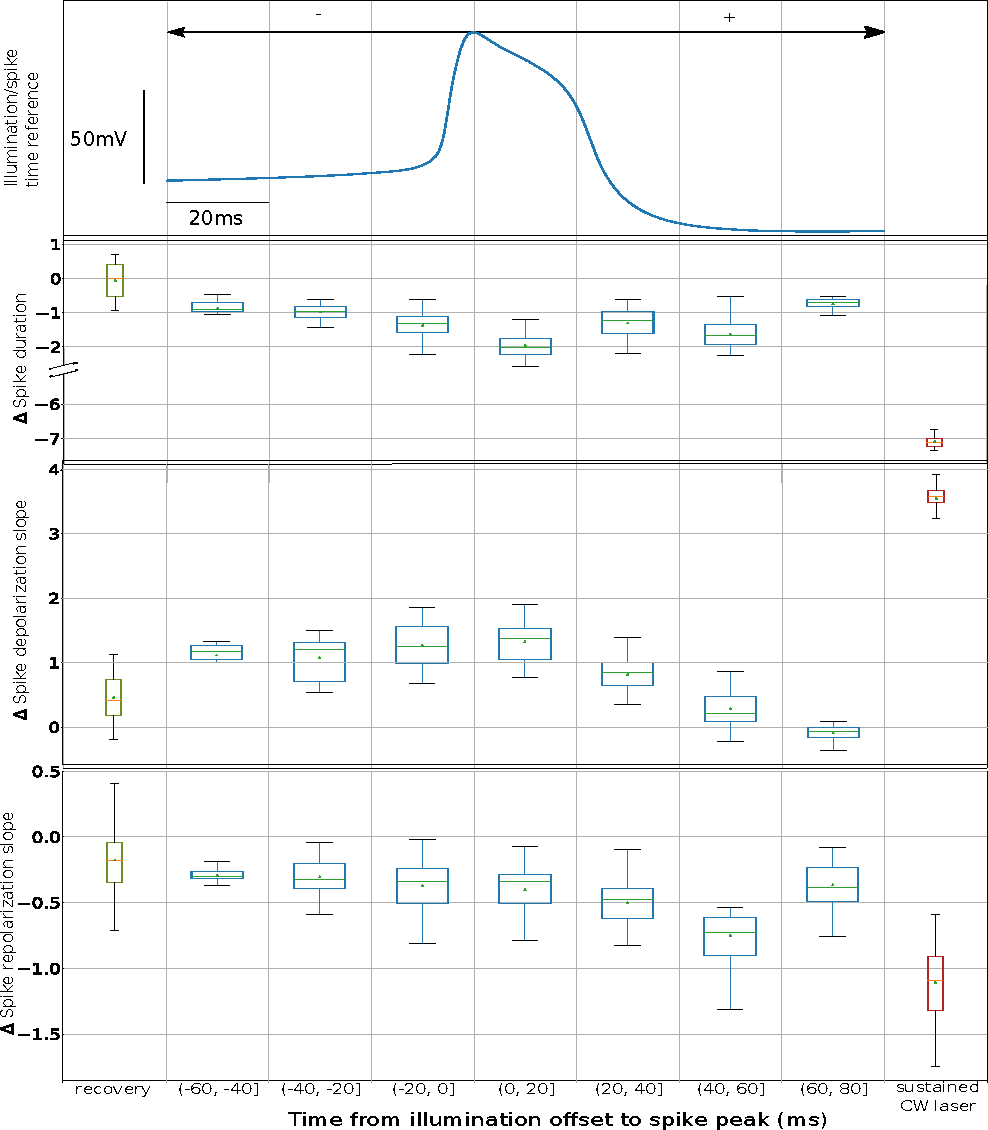
\includegraphics[width=0.8\textwidth]{img/laser/Figure6.pdf}
	\caption{Study of the laser effect at different stages of the spike waveform with an activity-dependent stimulation protocol. The panels quantify the change induced by the laser stimulation at distinct illumination offsets, --time intervals from the end of the illumination to the peak of the spike--. Top panel shows a spike waveform from the experiment as a time reference for the offset --time 0 corresponds to the spike peak. Boxplots represent the difference of each metric with respect to the control. All illumination intervals, pictured in the blue boxes, had the same duration of 58 ms and spikes were grouped by the illumination offset. Recovery and continuous laser reference are also shown in green and red boxes at left and right in the figure, respectively. The spike metrics selected here were duration, depolarization and repolarization slopes, --second, third and fourth rows, respectively.}
	\label{fig:activity dependent}
\end{figure}

Figure \ref{fig:activity dependent} shows the outcome of the application of this closed-loop protocol, with a stimulation interval lasting 58 ms. The time line in the figure represents the offset of the illumination, i.e., the time that corresponds to the end of an illumination interval to the peak of the action potential (see an illustration exemplifying the illumination offset in Fig. \ref{fig:offset_example}). The offsets were in the range from 60 ms before the action potential peak up to 80 ms after its occurrence (this wide range is required because of the natural slow dynamics of \textit{Lymnaea stagnalis}'s neurons). Each row in the figure represents the change in relation to the mean of the respective control trials for every illumination range. The change is represented for the three metrics in which we observed modulation during sustained illumination --duration, repolarization and depolarization slopes, respectively--. The different stimulation intervals are grouped by the time offset from the illumination to the peak of the action potential. The spike shown in the figure is plotted as a reference of the phase of the action potential in which the illumination finished. Recovery and sustained laser references are also represented at the left and right of each row, in green and red, respectively. For the three metrics here displayed, we can see how as the illumination offset got closer to the spike, the change was larger, and then recovered as the illumination interval covered less the action potential, resulting in an arch shape trend. Although this trend is visible for the three parameters characterized, it is manifested to a different degree in each of them. Note also that there was a temporal shift of the laser effect depending on the instant of stimulation. The maximum change value and the initialization of the recovery was different for the depolarization and for the repolarization. The effect on each of these metrics directly depended on the spike phase when the laser was illuminating the neuron. Thus, this variation of the laser effect points to a distinct modulation on each channel. The magnitude of the change under the sustained laser stimulation was larger than that observed at any of the phases addressed with the activity-dependent protocol. This may be caused by a heating delay during the stimulation, although there was no difference between the first and last spike in the sustained laser, the opening time of the laser shutter might have been smaller than the heating time necessary for the neuron to reach the maximum effect.

\begin{figure}[htb!]
	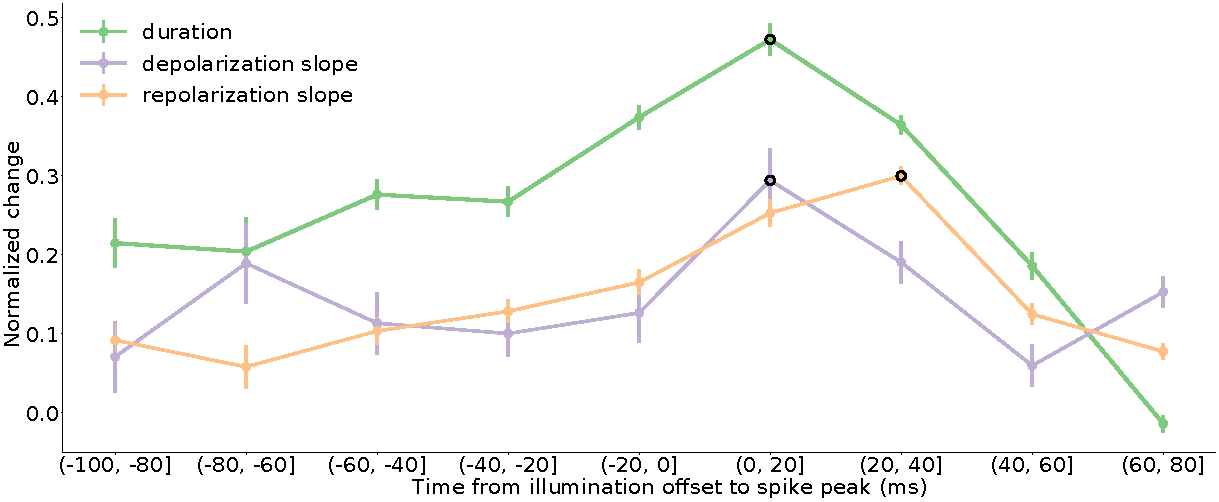
\includegraphics[width=\textwidth]{img/laser/Figure7.pdf}
	\caption{Normalized change for grouped values of spike duration, depolarization and repolarization slopes at distinct illumination offsets in the activity-dependent stimulation protocol. Each value in each group was normalized to the mean of its corresponding day controls as minimum value and the mean of the continuous laser recordings for each day as the maximum value. The maximum value for each metric is marked by a black circle. }
	\label{fig:activity dependent error mean }
\end{figure}

Figure \ref{fig:activity dependent error mean } agglutinates the results from 5 different closed-loop experiments, all of them normalized to the mean of the control and sustained laser references for each day, as minimum and maximum values, respectively. The arch trend is maintained. Again, note that the maximum effect for each spike metric occurs at a different stage. For the depolarization, the maximum change was found at the range of -20 to 0 ms, which corresponds to a stimulation during the whole depolarization. A fast rise when the illumination ceased right after the spike can be seen (i.e (0-20] range), since it corresponded to a stimulation during the depolarization and repolarization. In the repolarization, this trend was slightly delayed, reaching the maximum difference from the control at (20-40]. Such changes were also reproduced in the duration. This points to a modulatory effect of the laser depending on the stimulation instant. Previous to -20 ms, the laser was illuminating the neuron while all ionic channels were starting to activate, specially those involved in the process of the depolarization. However, those channels involved in the repolarization and hyperpolarization were also active earlier than the peak. This is why we can see a difference in all three metrics even at the early ranges of the action potential generation (e.g. -80 ms).

Using the activity-dependent protocol we were able to assess the neural activity at different stages of its dynamics in a controlled way. The results from these experiments showed that it is possible to modify the action potential generation in a temporally precise manner and that the effect of the CW-NIR laser illumination is dependent on the instant of the stimulation. This sets the basis for assessing the biophysical sources of the effect impacting distinct channels without modifying the system condition. Also, it is a proof of concept demonstrating the possibility of developing laser stimulation protocols driven by specific neural activity events in an accessible and freely available real-time tool.
